\documentclass[border=10pt]{standalone}
\usepackage{tikz}
\usetikzlibrary{arrows.meta, positioning, shapes.geometric, calc}

\begin{document}
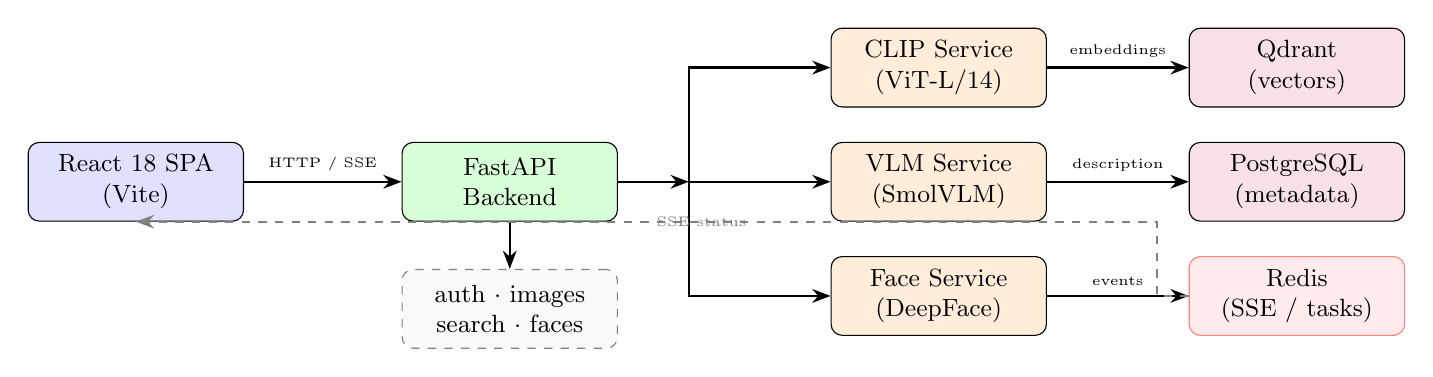
\begin{tikzpicture}[
  node distance=0.65cm and 1.8cm,
  box/.style   ={draw, rounded corners=4pt, text width=2.5cm,
                 minimum height=1.0cm, align=center, font=\small},
  dbox/.style  ={draw=gray, rounded corners=4pt, text width=2.5cm, dashed,
                 minimum height=1.0cm, align=center, font=\small, fill=gray!5},
  arr/.style   ={->, >=Stealth, thick},
  darr/.style  ={->, >=Stealth, thick, dashed, gray},
]

%% ---- Column 1: Client ----
\node[box, fill=blue!12] (fe) {React 18 SPA\\(Vite)};

%% ---- Column 2: Backend ----
\node[box, fill=green!15, right=2.0cm of fe] (api) {FastAPI\\Backend};
\node[dbox, below=0.6cm of api] (r1) {auth $\cdot$ images\\search $\cdot$ faces};

%% Bus fork point (midway between api and services)
\coordinate (bus) at ($(api.east)+(0.9,0)$);

%% ---- Column 3: AI Services (vertically centred around api) ----
\node[box, fill=orange!15, right=1.8cm of bus, yshift= 1.45cm] (clip) {CLIP Service\\(ViT-L/14)};
\node[box, fill=orange!15] (vlm)  at (clip |- api)                      {VLM Service\\(SmolVLM)};
\node[box, fill=orange!15, right=1.8cm of bus, yshift=-1.45cm] (face) {Face Service\\(DeepFace)};

%% ---- Column 4: Data Stores (each aligned with its service) ----
\node[box, fill=purple!12, right=1.8cm of clip] (qdrant) {Qdrant\\(vectors)};
\node[box, fill=purple!12] (pg)    at (qdrant |- vlm)  {PostgreSQL\\(metadata)};
\node[box, draw=red!50, fill=red!8] (redis) at (qdrant |- face)  {Redis\\(SSE / tasks)};

%% ---- Arrows ----
%% Client <-> Backend
\draw[arr] (fe.east) -- node[above, font=\tiny]{HTTP / SSE} (api.west);
%% Backend -> Routers
\draw[arr] (api.south) -- (r1.north);
%% Backend -> Bus -> Services (clean single fork)
\draw[arr] (api.east) -- (bus);
\draw[arr] (bus) |- (clip.west);
\draw[arr] (bus) |- (vlm.west);
\draw[arr] (bus) |- (face.west);
%% Services -> Stores
\draw[arr] (clip.east) -- node[above, font=\tiny]{embeddings} (qdrant.west);
\draw[arr] (vlm.east)  -- node[above, font=\tiny]{description} (pg.west);
\draw[arr] (face.east) -- node[above, font=\tiny]{events} (redis.west);
%% Redis SSE back to client (dashed)
\draw[darr] (redis.west) -- ++(-0.4,0) |- node[font=\tiny, right, near end]{SSE status} (fe.south);

\end{tikzpicture}
\end{document}
